\fakesection{Een Aanbevelingssysteem voor Films}

%%%
%%%
%%%

\fakesubsection{Opdracht 1}

We laden de dataset in met de \texttt{load} functie. De uitvoer staat weergegeven in figuur \ref{fig:op1}.

\vspace{0.3cm}
\begin{figure}[h]
\centering
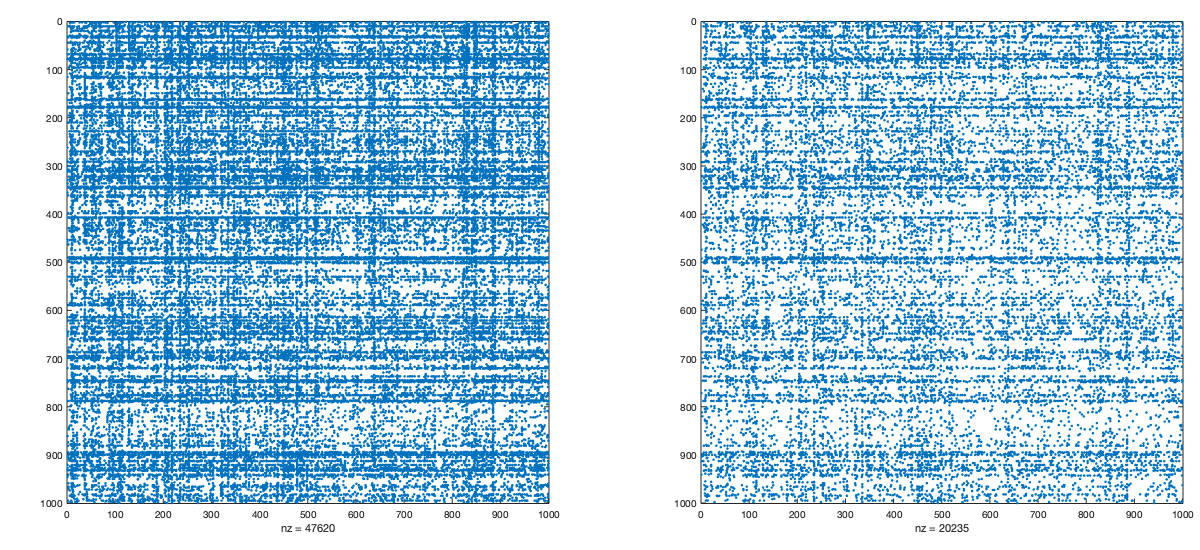
\includegraphics[width=0.5\textwidth]{res/op1.png}
\caption{Grafische voorstelling van ijle matrices $R$ en $T$.}
\label{fig:op1}
\end{figure}

\begin{lstlisting}
set(0, 'defaultFigurePosition', get(0, 'Screensize')); % Figuren vullen scherm
load('MovieLens_Subset.mat');
subplot(1,2,1)
spy(R(1:1000,1:1000))
subplot(1,2,2)
spy(T(1:1000,1:1000))
\end{lstlisting}

%%%
%%%
%%%

\fakesubsection{Opdracht 2}

De volle matrix \texttt{full(R)} neemt 220388224 bytes ($\approx 210$MB) in beslag. Voor de ijle matrix \texttt{sparse(R)} lijkt het op het eerste gezicht 18525728 bytes ($< 18$MB) te zijn. MatLab verbruikt echter iets meer dan dat. Als men de juiste formule gebruikt voor het geheugenverbruik van ijle matrices \footnote{\textit{\texttt{MATLAB} gebruikt het \texttt{CSC} formaat voor ijle matrices : ``Even though \texttt{MATLAB} is written in \texttt{C}, it follows its \texttt{LINPACK} and \texttt{Fortran} predecessors and stores full matrices by columns. This organization has been carried over to sparse matrices. A sparse matrix is stored as the concatenation of the sparse vectors representing its columns. Each sparse vector consists of a floating point array of nonzero entries (or two such arrays for complex matrices), together with an integer array of row indices. A second integer array gives the locations in the other arrays of the first element in each column. Consequently, the storage requirement for an $m\times n$ reals parse matrix with $nnz$ nonzero entries is $nnz$ reals and $nnz+n$ integers. On typical machines with 8-byte reals and 4-byte integers, this is $12nnz+4n$ bytes.''} \cite{Gilbert1992}} :
$$12\times nnz+4\times n$$
Dan komt men uit op bijna 14 miljoen bytes. Op mijn computer was het totaal meer dan 18,6 miljoen omdat gehele getallen 8 bytes innemen.

\begin{figure}[h]
\centering
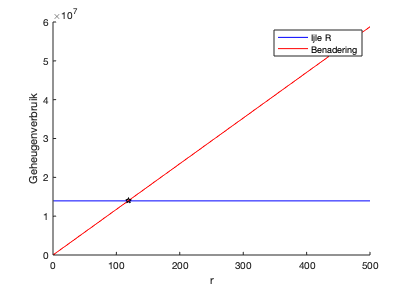
\includegraphics[width=0.5\textwidth]{res/op2.png}
\caption{Geheugenverbruik voor ijle matrix $R$ en lagerangsbenadering. Het snijpunt bevindt zich in $r\approx 119$.}
\label{fig:op2}
\end{figure}

\begin{lstlisting}
[m,n] = size(R);
ratings = nnz(R);
int_mem = 4;
double_mem = 8;
max_r = 500;
%
fprintf('Geheugenruimte full(R) : %i\n', m * n * double_mem)
%
size_sparse_naive = ratings * (int_mem * 2 + double_mem);
size_sparse = 12 * ratings + 4 * n;
fprintf('Geheugenruimte sparse(R) : %i\n', size_sparse)
%
fullR = full(R);
fprintf('Matlab zelf gebruikt respectievelijk %i en %i bytes.\n', whos('fullR').bytes, whos('R').bytes)
%
r = 1:max_r;
size_approx = (m + n) * double_mem * r;
snijpunt_r = size_sparse / ((m + n) * double_mem);
fprintf('Snijpunt in r = %i\n\n', snijpunt_r)
%
hold on
plot(r, repmat(size_sparse,1,max_r), 'b-')
plot(r, size_approx, 'r-')
plot(snijpunt_r, size_sparse, 'kp')
xlabel('r')
ylabel('Geheugenverbruik')
legend('Ijle R', 'Benadering', 'Location', 'northeast') 
\end{lstlisting}

%%%
%%%
%%%

\fakesubsection{Opdracht 3}



%%%
%%%
%%%

\fakesubsection{Opdracht 4}



%%%
%%%
%%%

\fakesubsection{Opdracht 5}

